\chapter{Schluss}
\label{chap:schluss}

\section{Strategie}

Im die PEST-Analyse zeigt, dass Smoilet in der Schweiz keinen speziellen Regulierungen unterliegt. Eine grosse Gefahr ist die direkte Konkurrenz durch etablierte Player auf dem Toilettenmarkt. Wir wollen diese Problematik aber entsch�rfen in dem wir von Anfang an auf eine Kooperation mit einem m�glichen Konkurrenten hinarbeiten.

\section{Markt}

Sp�ltoiletten sind weltweit verbreitet und der Absatzmarkt riesig. Jedoch ist die Einstellung zur Toilette stark von Kulturellen Aspekten gepr�gt und unterscheidet sich regional stark. Wir m�ssen bei der Marktbereitung jeweils penibel darauf achten den entsprechenden Markt richtig zu bearbeiten. Das Produkt soll in zwei Varianten erh�ltlich sein wobei f�r jede Variante ein unterschiedlicher Absatzkanal vorgesehen ist. Das Produkt soll erst einen Techie-Lifestyle vermitteln mit steigender Maturit�t aber zum zuverl�ssigen Produkt weiterentwickelt werden.

\section{Finanzen}

Ziel des Crowdfundings liegt nicht prim�r in der Umsatzsteigerung, sondern in der Gewinnmaximierung durch Kostenersparnisse in Bezug auf Werbung und Kundensuche. In unserer Kostenrechnung stellten wir fest, dass die reine Finanzierung durch Crowdfunding nicht realistisch ist. Zur L�sung dieses Problems haben wir zwei Varianten erarbeitet. Von welchen wir die Variante ,,Startfinanzierung durch Investoren`` bevorzugen.

\section{Weiteres Vorgehen}

Unsere Strategie sieht einen streng Timeboxed Ansatz vor. Wichtig dabei sind die strikten Meilensteinen. Sollte ein Meilenstein nicht erreicht werden, brechen wir das Projekt ab.

\begin{figure}[H]
	\centering
	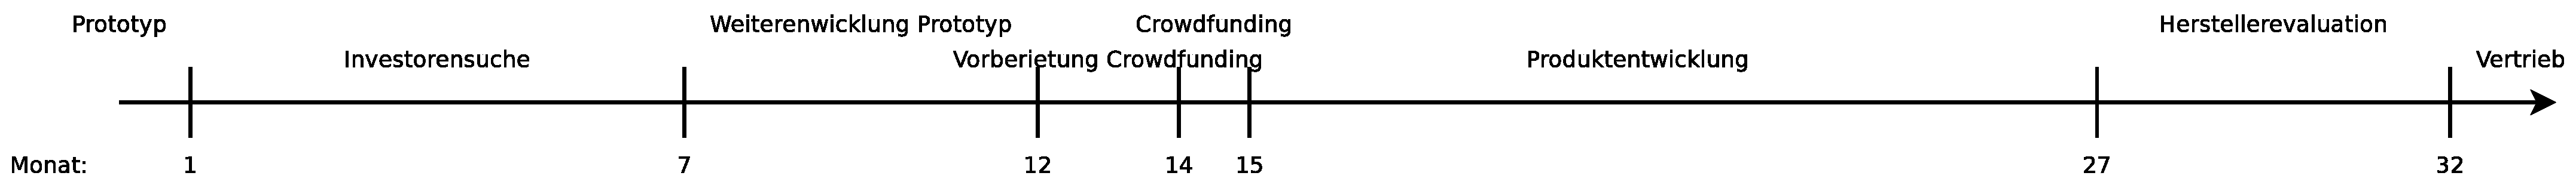
\includegraphics[width=\textwidth]{bilder/timeline}
	\caption{Timeline}
	\label{fig:timeline}
\end{figure}

\paragraph{Prototyp} Entwicklung eines Protoypen der die grunds�tzliche Machbarkeit aufzeigt. Ziel der Phase ist es einen Tweet beim Sp�len einer herk�mmlichen Toilette auszul�sen.

\paragraph{Investorensuche} Wir suchen mindestens einen Geldgeber der uns gen�gend unterst�tzt damit wir uns L�hne bis zur Vertriebsphase auszahlen k�nnen. Weiter soll in dieser Phase mindestens ein Partner f�r die OEM-Variante evaluiert werden.

\paragraph{Weiterentwicklung Prototyp} Wir entwickeln den Prototyp soweit weiter, dass dieser in der Crowdfunding-Phase Erfolg haben kann. Wir legen speziell Wert darauf die einfache Integration zu f�rdern und eine ansprechendes Design zu entwickeln. Ziel dieser Phase ist es einen ersten Anwender zu finden welchen wir vom Produkt �berzeugen k�nnen, so dass dieser das Produkt selbst nach dieser Phase installiert l�sst.

\paragraph{Vorbereitung Crowdfunding} Wir setzen eine Internetpr�senz und einen Social-Media auftritt auf. Ziel dieser Phase ist es, dass ein m�glicher Interessent auf eine Website mit Video verlinkt werden kann.

\paragraph{Crowdfunding} Ziel ist es das Funding-Goal zu erreichen.

\paragraph{Produktentwicklung} Smoilet 2.0 wird zum vertriebsf�higen Produkt: Neben den im Crowdfunding versprochenen Features muss eine Dokumentation, diverse Anwendungsf�lle und die E-Commerce Plattform aufgebaut werden.

\paragraph{Herstellerevaluation} Wir evaluieren einen Hersteller der Smoilet 2.0 produziert.

\paragraph{Vertieb} Mit dem Geld der Crowdfunding-Kampagne wird eine erster Batch Smoilet 2.0 produziert. Dieser Batch beinhaltet ein Smoilet 2.0 f�r jeden G�nner sowie einige Ger�te die �ber OEM-Kan�le vertrieben werden. Mit dem Absatz des OEM-Verkaufes finanzieren wir den n�chsten Badge an Smoilet 2.0.




